

\documentclass[aspectratio=169, 12pt]{beamer}

%%%%%%%%%%%%
% Packages %
%%%%%%%%%%%%

\usepackage{ctex}
\usepackage[english]{babel}
\usepackage{packages/sleek}
\usepackage{packages/tweaks}
\usepackage{calligra} % thanks pakeage
\usepackage{graphicx}

%%%%%%%%%%%%%%%%
% Bibliography %
%%%%%%%%%%%%%%%%

\addbibresource{./resources/bib/references.bib}

%%%%%%%%%%%%%%
% Title-page %
%%%%%%%%%%%%%%


\title{公共经济学}
\subtitle{Public Economics}
\author[LIU ShHUAI]{刘 {  } 帅}
\institute{山西师范大学 {  } 经济与管理学院}
\date{\today}
\titlelogo{./resources/pdf/logo.png}
\framelogo{./resources/pdf/logo.png}

%%%%%%%%%%%%
% Document %
%%%%%%%%%%%%

\begin{document}

\maketitle

\begin{frame}[standout]
    第四章\par
    \addtolength{\parskip}{.4em}
    市场效率
\end{frame}

\begin{frame}[plain]
    \frametitle{重点问题}
    \begin{itemize}
        \item \textbf{当经济学家说经济是有效率的时候,这是什么意思?}
        \item \textbf{如果市场是有效率的,必须满足哪些条件?}
        \item \textbf{竞争在确保效率中扮演什么角色?}
    \end{itemize}
\end{frame}

\begin{frame}[plain]
    % \begin{multicols}{1}
    %   \frametitle{Outline}
    %   \tableofcontents[hideallsubsections]
    % \end{multicols}
    \frametitle{Outline}
    \tableofcontents[hideallsubsections]
    % \tableofcontents[currentsection]
\end{frame}

\section{一、竞争性市场中看不见的手}

\begin{frame}[plain]
    \frametitle{看不见的手}
    1776年,亚当斯密在现代经济学的第一部重要著作《国富论》
    中指出,竞争会使人在追逐私人利益(利润)时,追求公共利益,
    就像被一只\textbf{看不见的手(invisible hand)}左右:
    \par
    He intends only his own gain, and he is in this, as in many other cases, led by an invisible hand to promote an end which was no part of his intention. Nor is it always the worse for the society that it was no part of it. By pursuing his own interest he frequently promotes that of the society more effectually than when he really intends to promote it.
\end{frame}

\section{二、福利经济学与帕累托效率}

\begin{frame}[plain]
    \frametitle{福利经济学}
    \begin{block}{福利经济学的萌芽}
        斯密的利己主义利益观表明,人们为了追求个人利益,
        必然采取最有利于社会的方法,从而有效地促进社会利益的实现。
        这一思想成为福利经济学的基本分析工具。
    \end{block}
    \begin{block}{福利经济学的产生}
        1920年英国经济学家阿瑟·庇古出版了世界上第一本以《福利经济学》命名的著作,因此被称为“福利经济学之父”。庇古以“价值判断”的规范分析为基本方法,采用基数效用论,认为福利是人们消费商品和服务时获得的效用,福利可以用数字度量且可以加总,能够用货币计量的福利是经济福利,个人福利的总和是社会总福利。
    \end{block}
\end{frame}

\begin{frame}[plain]
    \frametitle{福利经济学}
    \begin{block}{庇古福利经济学}
        社会总福利的大小取决于国民收入总量和国民收入在社会成员之间的分配:国民收入总量越大,社会总福利越大。国民收入在社会成员之间的分配越是均等化,社会总福利越大。增加社会总福利的途径一是增加国民收入总量,二是实现国民收入在全体社会成员之间的均等化分配。
    \end{block}
    \begin{block}{福利经济学}
        福利经济学(welfare economics)是对经济体系的规范性分析,
        即经济运行中什么是“对”、什么是“错”等问题和资源配置如何影响经济福利的研究。  
    \end{block}
\end{frame}

\begin{frame}[plain]
    \frametitle{帕累托效率}
    在混合经济背景下,公共部门和私人部门的分工组合可以有多种状态,
    我们如何评价各种可供选择的混合呢?大多数经济学家都接受的一个标准是:帕累托效率。
    \begin{block}{帕累托效率}
        帕累托效率以伟大的意大利经济学家和社会学家维尔弗雷多帕累托的名字命名。
        \par
        如果没有人的境况变差,就不会有人的境况变好,具备这种特征的资源配置就是帕累托效率或者帕累托最优。
        经济学家通常所说的的效率就是指帕累托效率。
    \end{block}
\end{frame}

\begin{frame}[plain]
    \frametitle{帕累托效率}
    \begin{block}{帕累托改进}
        指市场资源配置资源的过程,增加一个人的福利,
不会减少其他人的福利,从而使社会总福利增加。
    \end{block}
    \begin{block}{帕累托效率与个人主义}
       帕累托效率标准有一个重要特性需要说明——个人主义。这包括两层意思。
       \begin{enumerate}
        \item \textbf{他只关心每一个人的福利,不关心不同人的相对福利,
        明显不关心不平等}
        \item \textbf{每个人对自身福利的感觉最重要。这与消费主权的一般
        原则一致。该原则认为,个人时自己需要什么、自己的最大利益是什么的最好裁判。}
       \end{enumerate}
    \end{block}
\end{frame}

\begin{frame}[plain]
    \frametitle{福利经济学基本定理}
    \begin{block}{福利经济学第一定理}
        是指在经济主体的偏好被良好定义,并满足以下三个条件时:
        1.充分竞争2.没有信息不对称 3.没有外部性,
        市场将会达到帕累托最优的竞争均衡,
        此时每个经济个体所达到的纳什均衡即为经济体的帕累托最优状态。
    \end{block}
    \begin{block}{福利经济学第二定理}
        是指在完全竞争的市场条件下,
        政府所要做的事情是改变个人之间禀赋的初始分配状态,
        其余的一切都可以由市场来解决。
        每一种具有帕累托效率的资源配置都可以通过市场机制实现。
        然而,纠正分布的尝试可能会引入失真,因此重新分布可能无法达到完全的最优性。
    \end{block}
\end{frame}

\section{三、分析经济效率}

\begin{frame}[plain]
    \frametitle{三个层面的效率}
    帕累托效率要求交换效率、生产效率和产品组合效率。
    \begin{itemize}
        \item \textbf{第一,经济必须实现交换效率,即不管生产什么产品,产品都要到评价最高的的人手里。}
        \item \textbf{第二,必须要有生产效率,在社会资源既定的情况下,如果一种产品的生产不下降,另一种产品的生产就不可能增加。}
        \item \textbf{第三,经济必须实现产品组合效率,产品必须满足个人需求。不会出现结构性供给过剩和供给不足。}
    \end{itemize}
\end{frame}

\begin{frame}[plain]
    \frametitle{效用可能性曲线}
    效用可能性曲线给出的是在一个人的效用水平既定时,
    另一个人所能达到的最大效用水平。
    \begin{figure}
        \centering
        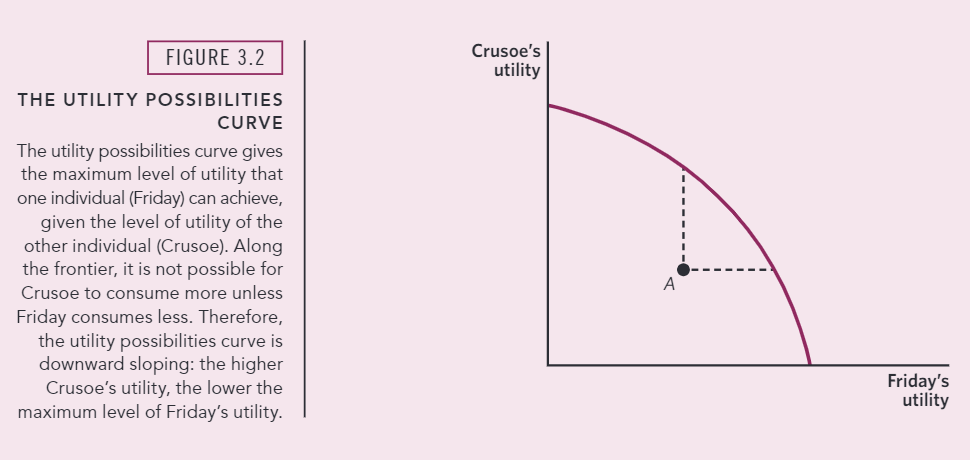
\includegraphics[width=1.0\textwidth]{./resources/figure/utilityc.png}
    \end{figure}
\end{frame}

\begin{frame}[plain]
    \frametitle{效用可能性曲线}
    福利经济学第一定理是说,竞争性经济沿着效用可能行边界运行。
    \par
    福利经济学第二定理是说,只要我们适当地重新分配初始禀赋,我们就能利用竞争性市场达到效用可能性边界上的任何一点。
\end{frame}

\begin{frame}[plain]
    \frametitle{交换效率}
    交换效率涉及产品分配。给定一组可得产品,交换效率表明了这组产品的
    这样一种分配状况,即如果没有人的境况变差,就没有人的境况变好。因此,
    交换效率要求没有交易余地或使双方的境况都变好的交换。
    \begin{figure}
        \centering
        \begin{minipage}{0.3\linewidth}
            一个人为了换取一单位其他商品而愿意放弃一种商品的数量,称为边际替代率。
            交换效率要求所有人的边际替代率都相同。
        \end{minipage}%
        \begin{minipage}{0.7\linewidth}
            \centering
            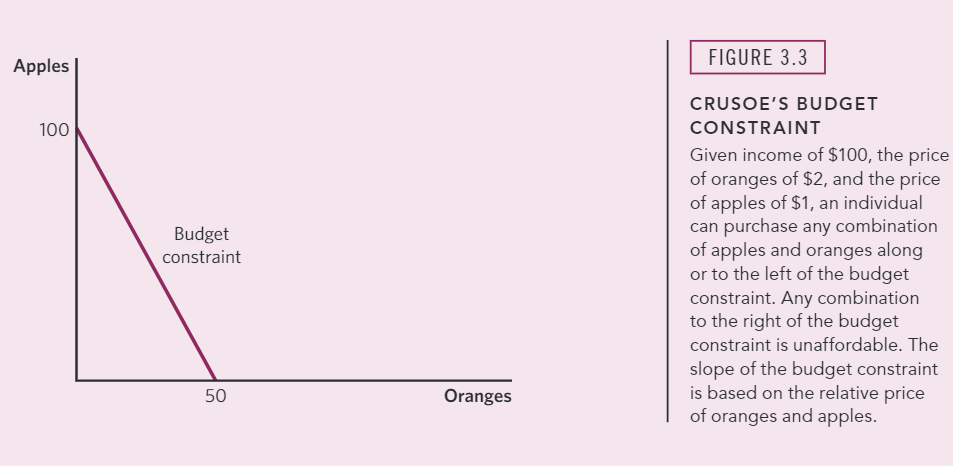
\includegraphics[width=1.0\textwidth]{./resources/figure/budget.png}
        \end{minipage}
    \end{figure}
\end{frame}

% ---------------------------------------------------------------------------
\begin{frame}[standout]
    \begin{center}
        {\Huge\calligra Thanks!}
    \end{center}
\end{frame}
% ---------------------------------------------------------------------------

\end{document}
